% chapter format et style

%***********************
\section{Introduction}
%***********************


\rouge{
Ce présent document est écrit avec Latex (outil texmaker), avec le choix du langage anglais ce qui explique les titres les noms en anglais pour chapitre ou liste des tableaux. C'est très facilement modifiable.
Dans l'idéal ce document devrait être écrit en anglais car beaucoup d'entreprise exige des rapports uniquement en anglais, pour diffusion dans les filiales
internationales ou vers les clients ou les autorités de certifications internationales.
}



Il faut lorsqu'on rédige un document distinguer ce qui concerne le format de ce qui concerne le style.

On peut le voir assez facilement dans les logiciels de traitement de texte car ces deux notions se retrouvent dans deux menus différents, mais aussi parce qu'il est
très souvent possible de trouver des documents pré-formatés, ou avec des styles spécifiques. On parle de "templates" en anglais.


Le format concerne pour l'essentiel:
\begin{itemize}
\item La taille du document (A3, Bx, format américain)
\item La taille des marges droites/gauches, haut/bas
\item la taille des images, des figures, des tableaux, etc ...
\item l'interlignage (espacement entre les lignes)
\item la présence et la position des numéros de page
\item la présence d'informations prédéfinies dans la haut et le pied de page
\end{itemize}
Le format fait essentiellement référence à de la géométrie. 


\vs{0.5}

Le style concerne pour l'essentiel:

\begin{itemize}
\item Le choix des types de fontes, leur taille pour un chapitre, une section, un paragraphe, le corps du texte
\item Les couleurs
\item l'ajout d'éléments de mise en valeur (cadre, traits épais de séparation, ...)
\item Le choix de l'écriture des légendes de figures et de tableaux,
\item la façon de présenter les équations, leur numérotation
\end{itemize}




%************************
\section{Mise en forme}
%************************








\begin{figure}[h]
  \begin{center}
  \input{Figures/configurations.pdf_tex}
  \caption{ Wind turbine rotor and propeller stream tube.}
  \label{fig:configs}
  \end{center}
\end{figure}



 



\section{style}


% **********************************************
\subsection{Hauteur du texte, aération, couleur}
% **********************************************

Le premier coup d'oeil sur un document va tout de suite donner envie de le lire ou 
de ne pas le lire. Pour cela il faut respecter quelques données de base:
\begin{itemize}
\item Le document doit posséder des marges (haut, bas, droite, gauche) respectables, mais sans exagération, couramment de 1 à 2 cm.

\item La taille du texte doit être 11 ou 12 points. 
10 points est une taille trop petit pour un document, c'est fatiguant à la lecture sur papier et mauvais pour les yeux. 14 points voir plus donne l'impression qu'on a essayé  d'allonger le rapport en augmentant la taille du texte.

\item L'écartement entre les lignes qu'on appelle interligne est toujours à la base de 1. Si on n'imprime pas le document, il faut mieux l'augmenter à 1.25 ou 1.5. Le document devient beaucoup plus lisible et donc appréciable. On peut passer localement à 2, par exemple pour les tableaux.

\item Le texte à l'intérieur des paragraphes soit être justifié c'est-à-dire qu'il doit prendre toute la largeur de la page sans les marges.
 C'est une option basique de tous les éditeurs de texte.\footnote{Des spécialistes indiquent qu'en fait c'est mauvais pour les dysléxiques et propice à se tromper de ligne, par rapport à des lignes irrégulières.}
 
\item On évite les demi-pages ou 1/4 ou 3/4 de pages blanches. Donc on ne change pas de page à chaque section.

\item On peut ajouter de la couleur dans un document, mais il faut mieux choisir un thème ou une couleur fondamentale et la déclinée plus ou moins foncée ou claire. Il faut éviter d'en ajouter de trop pour éviter l'effet arc-en-ciel.

\item Autrement on peut utiliser les fontes \textbf{épaisses (bold)} et \textit{italique} si on veut mettre un mot ou un morceau de phrase en valeur.

\item \texttt{Changer de fonte} peut aussi être un bon moyen.
\end{itemize}

% ***************************************************************
\section{Présentation et mise en forme des éléments importants}  
% **************************************************************   

Trois éléments se retrouvent systématiquement dans un rapport scientifique:
des équations, des figures et des tableaux.

Leur présentation suit des règles relativement strictes. 



% *********************************************
\subsection{Equations et symbôle mathématiques}
% **********************************************

% Equations

On utilise très souvent des équations ou des symbôles mathématiques  dans un document scientifique. 
Il suffit d'ouvrir  un livre ou un article pour voir de bons exemples. 

Il faut distinguer différentes configurations lorsqu'on introduit des équations ou bien des symbôles mathématiques:

\begin{itemize}
\item les équations sont au milieu du texte
\item les équations sont séparées du texte
\end{itemize}



Observer l'exemple suivant:


\textit{
L'accélération $a$ est définie comme la dérivée de la vitesse $v$ par $a = \dot v$. On peut aussi l'écrire sous la forme
$a = dv/dt$ ou bien $a = \frac{dv}{dt}$. Finalement on peut préférer la forme $a =\dfrac{dv}{dt}$ ou bien $\dsp v = \int a(t) dt$.
Si on l'écrit sur une ligne à part on a alors:
}

\begin{equation}
\dsp a = \der{v}{t}
\label{eq:acceleration}
\end{equation}



Séparer l'équation met en évidence une relation spécifique très utile à connaître. L'équation au milieu du texte correspond plus à
un rappel d'une définition ou d'une quantité déjà bien connue. Le choix de la hauteur de la formule joue un rôle sur sa mise en valeur
et sa lisibilité au milieu du texte en modifiant ou pas l'interlignage.

Il est plutôt préconisé de choisir la même hauteur que le texte pour les relations mélangées à celui-ci.
 




Quelques recommandations très simples 

\begin{itemize}
\item Centrer les équations sur une ligne
\item Aligner sur le signe = quand il y a plusieurs équations
\item Bien gérer les espacements horizontaux et verticaux
\item Numéroter uniquement les équations que vous appellerez dans le texte
\item Quand on fait des développements avec des détails, préférer les mettre dans un annexe et ne mettre dans le corps du texte qu'un ou deux étapes (aucune évidente, comme les simplifications basiques)
\item On encadre rarement les équations, mais parfois cela fait partie du style du document, pour celles qui sont vraiment importantes.
\end{itemize}

On pourra donc analyser la mise en forme des équations suivantes, présentées de la meilleure façon à la pire.

\begin{equation}
\dsp
x (t) ~=~\dfrac{1}{2}~\textrm{e}^{k t}~\sin\omega t, \qquad \der{x}{t}~=~\dfrac{1}{2}~ \rm{e}^{k t}~(k~\sin \omega t~-~\omega~\cos\omega t)
\label{eq:xv1}
\end{equation}


\setstretch{2}
\begin{eqnarray}
\dsp
x (t) &=&\dfrac{1}{2}~\textrm{e}^{k t}~\sin\omega t \label{eq:xv2a} \\
\dsp \der{x}{t}&=& \dfrac{1}{2}~ \rm{e}^{k t}~(k~\sin \omega t~+~\omega~\cos\omega t)
\label{eq:xv2b}
\end{eqnarray}
\setstretch{1}

\begin{equation}
\begin{array}{l}
x(t) = 1/2 \textrm{e}^{k t} \sin\omega t\\
\der{x}{t}=\frac{1}{2}\rm{e}^{k t}(k~\sin \omega t+\omega\cos\omega t)
\end{array}
\label{eq:xv3}
\end{equation}

\begin{equation}
x(t) = e^{k t} sin(\omega t)/2,   \der{x}{t}=e^{k t}(k sin \omega t+\omega\cos\omega t) / 2
\label{eq:xv4}
\end{equation}

Commentons:

\begin{itemize}
\item Pour l'équation \eqref{eq:xv1}:
	\begin{itemize}
	\item on a mis des espaces avant et après le signe "=" et avant les fonctions $\cos$ et $\sin$
    \item les fonctions sont en lettres romanes alors que les variables sont en italiques
    \item On n'a enlevé les parenthèses évidentes dans le cosinus et le sinus.	
    \item On a mis les deux équations sur une seule ligne, car cela correspond à une définition d'une fonction et de sa dérivée temporelle, mais l'espacement
    entre les deux équations est suffisamment important pour les mettre en évidence.
	\end{itemize}
\item La forme de la seconde équation \eqref{eq:xv1} est aussi très correcte.
  En plus du cas précédent on a ajouté des numéros à chaque équation, et elles sont
alignées sur le signe "=". On a aussi augmenté l'interlignage pour une meilleure lisibilité.

La numérotation pourrait aussi être de la forme 3.3a et 3.3b. Mais ce n'est pas absolument nécessaire.

\item L'équation \eqref{eq:xv3} n'est pas très belle. Le facteur 1/2 est écrit de deux façons différentes, les signes "=" ne sont pas alignés,  la dérivée 
et le facteur 1/2 apparaîssent  tout petit. Enfin la gestion des espacements est aléatoire.

\item La dernière équation est peu lisible et les fonctions apparaissent en italique comme les variables. Le facteur multiplicateur 1/2 apparaît à la fin. En général
on met les constantes au début de l'équation.
\end{itemize}


Enfin \textbf{il faut respecter les règles des mathématiques} en mettant des parenthèses quand c'est nécessaire.
 On trouve trop souvent l'erreur 
$f = \omega~/~2~\pi$ au lieu de $f = \omega~/~(2~\pi)$. La première écriture signifie mathématiquement $f = 0.5~\omega~/~\pi$
et elle est totalement fausse pour le lien entre pulsation et fréquence. 






     
% **************************
\subsection{Figures}
% **************************

\begin{figure}[htb]
\begin{center}
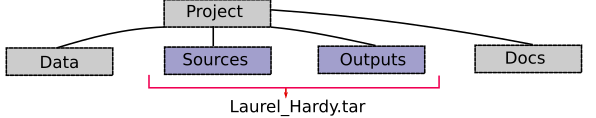
\includegraphics{Figures/architecture.png}
\caption{Exemple de figure: architecture du projet}
\label{fig:2}
\end{center}
\end{figure}

Des figures très soignées ou très jolies impressionnent toujours le lecteur.

Il faut pour cela apprendre à maîtriser les options graphiques des langages comme Matlab ou Python.

 Encore mieux, pour les plus experts, il faut savoir utiliser des logiciels de traitement d'images, comme GIMP par exemple, et des logiciels graphiques vectoriels comme Inkscape. Ces deux logiciels permettent de faire des choses très complexes comme introduire du texte ou des équations dans une figure ou images, ou de superposer des graphes à des images, ou d'autres choses plus complexes. Il faut du temps pour apprendre ces logiciels, mais c'est un investissement rentable pour toute la carrière, en plus des études. 

\subsubsection{Figures en général}

Il existe trois types génériques de figures:
\begin{itemize}
\item des dessins qui illustrent quelque chose, une géométrie, une configuration, une expérience, des mesures,  etc ...
\item des images
\item des graphiques contenant des représentations de résultats numériques sous différentes formes.
\end{itemize}

Parfois une figure est un mélange des trois cas.

Pour tous ces types la figure doit :
\begin{itemize}
\item avoir un numéro  (souvent automatique avec les éditeurs de texte)
\item avoir une légende qui indique clairement le contenu de la figure. La légende peut aller jusqu'à 4 ou 5 lignes parfois, si elle est très descriptive
\item  être centrée sur la largeur de page
\item  avoir une hauteur de 3 à 7 cm. Exceptionnellement elle peut prendre une moitié ou une hauteur totale de page, notamment quand une figure est composé de plusieurs sous-figures.
\item avoir une bonne définition en pixels. Attention aux copies d'écran ou aux images basses définitions qu'on récupère à droite ou à gauche, et qui donne au final un rendu flou
\item respecter le rapport d'aspect de la figure ou image originale. Le rapport d'aspect est le rapport hauteur/largeur. Sinon l'image à l'air d'être étirée dans une direction, ce qui donne un rendu affreux
\item  avoir des  textes  lisible sà l'échelle  100\%, surtout  s'ils sont importants pour comprendre la figure.
\item être positionnée judicieusement dans le document, c'est-à-dire proche de l'endroit où on la décrit. Si ce n'est pas possible, cela indique qu'il n'y a pas assez de commentaires sur les figures et que certaines sont inutiles ou à positionner dans une annexe. 
Deux autres conseils peuvent être donnés:
\begin{itemize}
\item En général on préfère mettre une figure en haut de page ou vers le milieu. 
\item On évite d'avoir une ligne ou deux de texte entre des figures, car en général le lecteur ne les verra pas.
\end{itemize}


\end{itemize}

\subsubsection{Graphiques scientifiques}

Pour les figures représentant des nombres, des fonctions ou  des isolignes ou autre,  il faut veiller à:
\begin{itemize}
\item avoir une légende sur l'axe des abscisses et très très souvent aussi sur l'axe des ordonnées
\item avoir une bonne visibilité des courbes. Cela implique un choix de couleurs, d'épaisseurs ou de taille de symbôles judicieux. 
\item éviter la surcharge de courbe. Au-delà de quelques courbes (3 à 5) on ne voit plus rien sur une figure, sauf si les courbes sont étagées. 
\item avoir une légende pour chaque courbe quand il y en a plusieurs
\item avoir l'échelle des couleurs quand on a des isobarres ou l'échelle des valeurs si possible, quand on a des isolignes.
\item avoir une taille de fonte lisible pour  des nombres et les textes
 sur les axes des abscisses, des ordonnées pour le  titre et les légendes
\item ajouter des lettres lorsqu'on a des sous-figures. Des hauteurs des sous-figures doivent rester décentes (supérieures à 1.5 ou 2 cm). 
\item ce que les échelles sur les deux axes soient choisies judicieusement de manière à ce que le graphique remplisse globalement le cadre. 
\item choisir correctement les axes, en semi log ou log-log ou échelles linéaires
en faisant attention aux signes des valeurs naturellement.
\item  ajouter une grille bien définie si on souhaite prendre des valeurs sur les courbes

\item comparer correctement des résultats lors de validation. On doit avoir par exemple quand c'est possible la courbe résultat et la courbe de référence sur le même graphe, et pas sur deux graphes côte à côte. Lors qu'on est obligé de comparer deux figures côte à côte il faut respecter les dimensions des figures, et avoir des valeurs identiques sur les deux axes, avec une grille.
\end{itemize}

Enfin, quand on fait un commentaire sur une figure, on doit \textbf{faire référence au numéro de la figure}. Le commentaire doit faire quelques lignes. La première chose est de décrire ce qui est représenté. Ensuite on commente les tendances, les variations, les points particuliers (maximun, minimun, discontinuités, ...)

Voici un exemple de commentaire :

La figure \ref{fig:1} représente l'expérience sur un anneau tourbillonnaire (a), un exemple de visualisation à un instant donné(b), et enfin une reconstruction 
de l'anneau tourbillonnaire dans un plan. ... bla bla ...

\bleu{On peut remarque que les nombres sur la figure (c) ont été agrandis et que les épaisseurs des traits sur toutes les figures ont été forcés.}

Deux remarques lorsqu'on veut conserver un graphe pour un rapport ou une présentation:

\begin{itemize}
\item En général dans tous les langages classiques comme Python ou Matlab, les épaisseurs des traits et les hauteurs des nombres par défaut sont optimisées pour la visualisation sur un écran (de grande dimension). Pour une sauvegarde et
une introduction dans un rapport il faut toujours définir les hauteurs et épaisseurs dans le programme et ne pas se contenter des valeurs par défaut. Il faut aussi tenir compte de la possible réduction de l'image dans le document.

\item En toute logique, pour une présentation orale des résultats il faut
refaire des figures spécifiques en augmentant encore la hauteur des textes et l'épaisseur des traits pour améliorer la visibilité via un vidéo-projecteur.
\end{itemize} 

Les figures doivent apparaître dans l'ordre où elles sont nommées. Par exemple ici, je me suis trompé  volontairement en parlant d'abord de la figure \ref{fig:1}
alors que la première à apparaître est la figure \ref{fig:2}.


 
\begin{figure}[htb]
\input{Figures/experiment.pdf_tex}
\caption{Vortex ring experiment and results \cite{Albagnac}, a) experimental set-up,b) example of picture, c) example of the velocity field.}
\label{fig:1}
\end{figure}


 


%**************************
\subsection{Table, tableaux}
%*************************


 
 
 


% Exemple de tableaux





Un  tableau permet de synthétiser des résultats issus de simulations numériques ou des valeurs expérimentales 
ou de fournir des paramètres en un coup d'oeil. 
Il contient donc toujours des informations jugées  essentielles sous la forme de données numériques ou de texte.

\begin{itemize}
\item Il est déconseillé de positionner des tableaux au milieu du texte lorsque cela diminue sa visibilité.
\item Il vaut mieux les insérer comme des figures avec un numéro et une légende.
\item Il ne faut pas oublier de positionner le tableau près de l'endroit où il est évoqué et de le nommer par sa référence
\item Un tableau doit rester sobre.  
 \item On peut ajouter quelques couleurs par alternance, par lignes lorsqu'il y a beaucoup de lignes pour améliorer la lecture
 et minimiser les erreurs de lecture. On peut aussi procéder ainsi pour les colonnes.
\item Préférer un tableau avec des colonnes larges que des colonnes serrées et il faut  centrer le tableau sur la page.
\item le tableau devra être amélioré en ajoutant des couleurs et en augmentant les tailles de fontes 
pour une présentation en mode diapositive
\item s'il y a beaucoup d'information à faire passer, il faut mieux proposer plusieurs tableaux qu'un tableau illisible ou incompréhensible
\end{itemize}




\begin{table}[htb]

\vs{0.5}

\setstretch{1.4}
\small
\centering
\begin{tabular}{p{1.5cm}p{2.5cm}p{2.5cm}p{3.5cm}p{3cm}p{2cm} }
\Xhline{2pt}
Case    &      Fluid    & Velocity     & Reynolds number   &  Flow rate     & Length \\ 
        &               & $U$~[m/s]    & $Re$ in $10^6$  &  $q_m$~[kg/m$^3$] &  $\ell$~[mm] \\ \Xhline{1pt}
1       & Air           & $100$        &   $1.5$         &  $100$            &  $35.33$     \\
2       & Water         &  $\;\;10$        &   $0.1$         &  $\;\;78$             &  $\;\;5.24$  \\
\Xhline{2pt}
\end{tabular}
\caption{Premier exemple  de format de tableau (excellent).}           
\label{tab:exemple1}   
\normalsize
\setstretch{1}
\end{table}


Les tableaux tabs.~\ref{tab:exemple1}, \ref{tab:exemple2} et \ref{tab:exemple3} sont trois exemples qu'on peut rencontrer.

Commentons les.



\begin{enumerate}
\item Le premier tableau tab.~\ref{tab:exemple1} est rencontré dans les publications scientifiques. Il respecte les consignes suivantes:
		\begin{itemize}
		\item Il est sobre avec deux lignes épaisses pour délimiter le tableau dans le plan vertical et une ligne fine
		 qui démarque le titre des colonnes
		 \item Les grandeurs sont clairement décrites avec leur symbôle et leur unités physiques 
		 \item l'interlignage ou espacement vertical est suffisamment important pour améliorer la lisibilité
		 \item les valeurs ou textes sont positionnés à gauche et alignés (on peut aligner sur le . pour les nombres réels)
		 \item le tableau occupe presque la largeur de la page, les colonnes sont dimensionnées précisément.
		 \item le tableau est bien séparé du texte et ressort bien
		 \item on peut remarquer que la hauteur de fonte est légèrement inférieure à celle du texte principale, ce qui peut
		 permettre d'ajouter plus de colonnes et de lignes sans occuper trop de place.
		\end{itemize}
		
		C'est la référence à suivre.
		

		
\item Le second tableau tab.~\ref{tab:exemple1} est aussi acceptable mais souffre de quelques défauts:
		\begin{itemize}
		\item on ne connaît pas le sens des variables
		\item les unités sont répétées inutilement
		\item les colonnes sont trop serrées, elles n'occupent pas l'espace en largeur
		\end{itemize}	
		on peut ajouter qu'il n'y a pas de délimitation horizontale et que l'interlignage est très fort. Mais celà
		n'est pas nécessairement négatif.
		
		On peut alors rajouter le sens des variables dans la légende qu'il faut bien lire pour comprendre le tableau.
		
\begin{table}[htb]
\centering
\setstretch{2}
\begin{tabular}{c|cccc}
Case             & Fluid    & $U$               & $Re$                   &   $q_m$ \\ \hline\hline
1                & Air     & $100$~m/s        &   $1.5 \times 10^6$    &  $100$~kg/m$^3$                       \\
2                & Water   &  $10$~m/s        &   $0.1 \times 10^6$    &   $5$ ~kg/m$^3$      \\
\end{tabular}
\caption{Deuxième exemple de format de tableau (acceptable). La vitesse est notée $U$ et le débit massique $q_m$. }           
\label{tab:exemple2}   
\normalsize
\setstretch{1}
\end{table}
		
\item Le dernier exemple  tab.~\ref{tab:exemple1} est une représentation très basique des données sans aucune réflexion sur le rendu. Ils souffrent de tous les défauts possibles
	   qui sont le contraire des qualités du premier tableau. Il n'est en particulier pas nécessaire de marquer les lignes et
	   les colonnes quand c'est évident. Et il n'y ni unité, ni explication sur le sens des variables. Enfin les lignes et les colonnes sont très resserrées.
	   On peut aussi remarquer que le tableau n'est pas centré sur la page.
	   
	   Cette représentation est à proscrire!
	   
	   
\begin{table}[htb]
\begin{tabular}{|c|c|c|c|c|}
\hline
Case             & Fluid    & $U$          & $Re$                   &   $q_m$ \\ \hline
1                & Air     & $100$        &   $1.5 \times 10^6$    &  $100$    \\ \hline
2                & Water   &  $10$        &   $0.1 \times 10^6$    &   $5$      \\ \hline
\end{tabular}
\caption{Troisième exemple de format de tableau (le plus mauvais) }           
\label{tab:exemple3}   
\normalsize
\setstretch{1}
\end{table}
	   
\end{enumerate}


On peut aussi:

\begin{itemize}
\item ajouter de la couleur soit par ligne, soit par colonne, soit une ligne sur deux et une colonne sur deux pour encore améliorer la visibilité.
\item choisir une couleur unique avec une teinte foncée et claire pour éviter l'effet "arc-en-ciel"
\item encore jouer sur les épaisseurs des traits.
\item modifier les types de fontes par rapport à celle du texte principal pour insister sur le contenu des colonnes
\end{itemize}












 
 

% *******************************************************
\section{Styles spéciaux}
% *******************************************************

En fonction du contexte on peut appliquer des styles spéciaux pour mettre en avant 
des choses importantes. Il faut rester malgré tout sobre.

  

\Attention{Message d'avertissement avec une mention en anglais.}

 
  \Important{Il faut absolument éviter le plus possible les fautes de grammaire et d'orthographe ainsi que les erreurs typographiques.
  
  Pour cela il faut :
  \begin{itemize}
  \item utiliser les dictionnaires intégrés au logiciel de publication
  \item relire le rapport plusieurs fois, en laissant du temps (heures, jours) entre les lectures.
  \end{itemize}
  
  }
  
  


\section{Conclusion}